\documentclass[UTF8]{article}
\usepackage{ctex}
\usepackage{ulem}
\usepackage{dsfont}
\usepackage{amssymb}
\usepackage{amsmath}
\usepackage{graphicx}
\newtheorem{thm}{定义}[section]
\newtheorem{notation}[thm]{记号}
\newtheorem{lemma}[thm]{引理}

\makeatletter
\newcommand{\rmnum}[1]{\romannumeral #1}
\newcommand{\Rmnum}[1]{\expandafter\@slowromancap\romannumeral #1@}
\makeatother
\newcommand{\dperp}{\perp\!\!\!\perp}

\title{12 $\lambda{\rm D}$中的数学:第一个尝试\\Mathematics in $\lambda{\rm D}$: a first attempt\\[2ex]\begin{large}读书笔记\end{large}}
\author{许博}
\date{}

\begin{document}
\maketitle
	\section{先举个例子}
	\noindent
	第十一章中,我们在$\lambda{\rm D}$中表示了逻辑。在本章中,将转向数学(mathematics)。尽管逻辑的推导框架对数学至关重要,因为逻辑包含了推理的原则,但是数学本身要比单纯的逻辑多的多。
	
		本章以一个关于偏序集合的例子开始,即证明在这样的集合中只存在至多一个最小元。一个在集合$S$上的关系$R$如果满足自反性,反对称性和传递性,则这个关系是偏序的。\\
		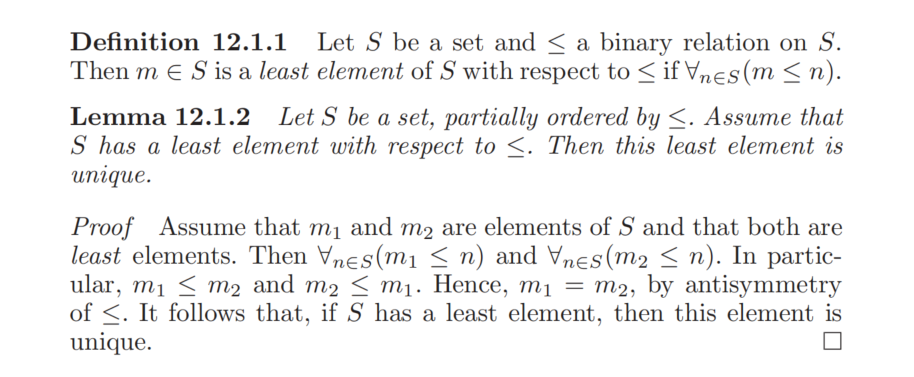
\includegraphics[width=0.93\linewidth]{"../imgs/12-1.png"}
		
		在$\lambda{\rm D}$中形式化这个证明:\\
		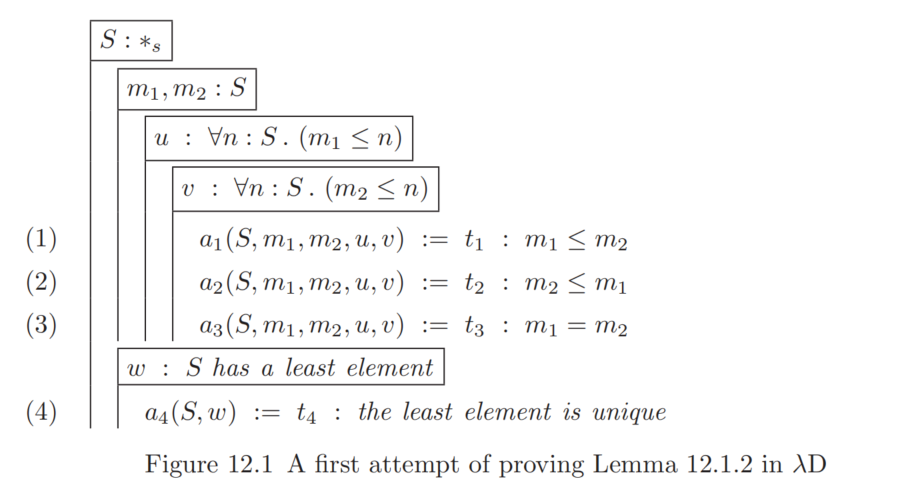
\includegraphics[width=0.93\linewidth]{"../imgs/12-2.png"}
		
		注意到其中存在的几个问题。有一些可以以直观的方式解决:\\
		- 符号`$\le$'表示在$S$上的一个任意的偏序关系。这些隐含的假设会在章节12.4中明确的表示。\\
		- 全称量词$\forall$在$\lambda{\rm D}$中被编码为$\Pi$。\\
		- 解决未知项$t_1$和$t_2$代表什么:应是$\forall$-消去规则的实例,所以令$t_1\equiv\forall{-el}(S,\lambda x:S.m_1\le x,u,m_2)$以及$t_2\equiv\forall{-el}(S,\lambda y:S.m_2\le y,v,m_1)$,或者简单地令$t_1\equiv um_2$以及$t_2\equiv vm_1$。
		
		剩下的问题似乎更加重要:\\
		$\it{Q1}$ 符号`='表示了基本的相等关系,作为数学中许多领域的基础,但尚未是我们系统的一部分,如何补足这点?\\
		$\it{Q2}$ 行(3)中$t_3$代表什么?\\
		$\it{Q3}$ 如何表达$S$拥有一个最小元?\\
		$\it{Q4}$ 如何表达最小元的唯一性?\\
		$\it{Q5}$ 如何证明最小元的唯一性,也即$t_4$是什么?
\end{document}
